\documentclass[aspectratio=43]{beamer}
\usetheme{Simple}

\usepackage[UTF8,fontset=fandol]{ctex}
\usepackage{graphicx}
\usepackage{amsmath}
\usepackage{amsfonts}
\usepackage{amssymb}
\usepackage{booktabs}
\usepackage{array}
\usepackage{xcolor}
\usepackage{xurl}
\usepackage{hyperref}
\usepackage{tikz}
\usetikzlibrary{arrows.meta, calc, positioning, shapes.geometric}
\setbeamertemplate{caption}[numbered]

\graphicspath{{Figures/}}

\def\meetingname{Research Presentation}
\title{AegisKV: Problem Formulation}
\subtitle{Three System Modules for Workflow-Aware KV Backup}
\author[Z Zhao]{Zhan Zhao}
\institute[HKBU]{Hong Kong Baptist University}
\date[2026.07.07]{\meetingname\\July 7, 2026}

\hfuzz=100pt
\hbadness=10000
\vfuzz=100pt
\vbadness=10000
\emergencystretch=\maxdimen

\definecolor{hkblue}{RGB}{24,76,133}
\definecolor{softblue}{RGB}{230,240,250}
\definecolor{softgreen}{RGB}{232,245,236}
\definecolor{softred}{RGB}{252,232,230}
\definecolor{softgray}{RGB}{245,246,248}
\definecolor{softyellow}{RGB}{255,247,220}

\newcommand{\smallcard}[2]{%
  \begin{beamercolorbox}[wd=\textwidth,rounded=true,shadow=false,sep=1.0ex]{block body}
    \textbf{#1}\par
    \vspace{0.25ex}
    \scriptsize #2
  \end{beamercolorbox}
}

\newcommand{\tightblock}[2]{%
  \begin{block}{#1}
    \footnotesize #2
  \end{block}
}

\begin{document}

\begin{frame}[plain]
  \titlepage
\end{frame}

\begin{frame}{Outline}
  \tableofcontents
\end{frame}

%------------------------------------------------------------
\section{Problem Formulation}
%------------------------------------------------------------

\begin{frame}{AegisKV 三个系统模块}
  \small
  AegisKV 仍按 2026.07.06 的思路建模：先识别 Critical Agent，再对 KV Segment 做 backup placement。
  \[
    \min \operatorname{AvgWCT}
    =
    \min \frac{1}{|\mathcal{W}|}\sum_{w\in\mathcal{W}}\operatorname{WCT}(w).
  \]

  \vspace{0.08cm}
  给定 workflow metadata、online agent state、KV Segment 与 runtime load，系统维护三个协同模块：

  \vspace{0.10cm}
  \begin{columns}[T,onlytextwidth]
    \begin{column}{0.32\textwidth}
      \smallcard{Module 1 / Alg. 1}{Critical Agent\\输出 $c_a(t)$}
    \end{column}
    \begin{column}{0.32\textwidth}
      \smallcard{Module 2 / Alg. 2}{Segment Placement\\GPU / Host / skip}
    \end{column}
    \begin{column}{0.32\textwidth}
      \smallcard{Module 3 / Alg. 3}{Backup HBM Cost\\输出 $\alpha$}
    \end{column}
  \end{columns}

  \vspace{0.12cm}
  \footnotesize
  Alg. 1 不评价某段 KV 本身，而是给 agent 一个 critical score；Alg. 3 只描述当前 HBM 是否适合 backup；Alg. 2 再把两者合并到 KV Segment placement。
\end{frame}

% \begin{frame}{模块耦合：Critical + Cost $\rightarrow$ Placement}
%   \small
%   \begin{center}
%   \begin{tikzpicture}[
%     node distance=0.45cm and 0.35cm,
%     box/.style={draw=hkblue, fill=softblue, rounded corners, align=center,
%                 font=\scriptsize, inner sep=4pt, minimum width=2.20cm,
%                 minimum height=0.70cm},
%     wide/.style={draw=hkblue, fill=softgreen, rounded corners, align=center,
%                  font=\scriptsize, inner sep=4pt, minimum width=2.55cm,
%                  minimum height=0.70cm},
%     arr/.style={-{Stealth[length=2mm]}, thick, draw=hkblue}
%   ]
%     \node[box] (wf) {Workflow DAG\\real trace};
%     \node[box, right=of wf] (a1) {Alg. 1\\$c_a(t)$};
%     \node[box, below=0.72cm of wf] (load) {Runtime load\\HBM state};
%     \node[box, right=of load] (a2) {Alg. 2\\$B_g, C_{\mathrm{hbm}}$};
%     \node[wide, right=0.80cm of a2] (a3) {Alg. 3\\tier$(s,t)$};
%     \node[wide, right=of a3] (safe) {Protected\\KV Segments};
%     \node[wide, below=0.72cm of safe] (recover) {Failure-time action\\GPU / Host / recompute};

%     \draw[arr] (wf) -- (a1);
%     \draw[arr] (load) -- (a2);
%     \draw[arr] (a1.east) -| (a3.north);
%     \draw[arr] (a2) -- (a3);
%     \draw[arr] (a3) -- (safe);
%     \draw[arr] (safe) -- (recover);
%   \end{tikzpicture}
%   \end{center}

%   \vspace{0.04cm}
%   \footnotesize
%   流程上，Alg. 1 只给 Alg. 3 提供 agent-level criticality；Alg. 2 只给 Alg. 3 提供 HBM cost / gate。Placement 是唯一做 KV Segment tier 决策的模块。
% \end{frame}

\begin{frame}{算法 1：Workflow Critical Path 与 WCT}
  \small
  单个 workflow 的 completion time 由 \textbf{critical path} 决定：

  \vspace{0.06cm}
  \[
    \operatorname{WCT} = \sum_{a' \in \pi_{\mathrm{crit}}} T(a')
    + \mathbf{1}[\mathrm{fail}(a)] \cdot T_{\mathrm{retry}}(a).
  \]

  \vspace{0.04cm}
  \footnotesize
  $\pi_{\mathrm{crit}}$：critical path agent 序列；
  $T(a')$：agent 执行时间；
  $T_{\mathrm{retry}}(a)$：failure 后 retry 开销。（当前基于静态 workflow，后续增加Criticality Predictor）

  \vspace{0.08cm}
  \begin{figure}
    \centering
    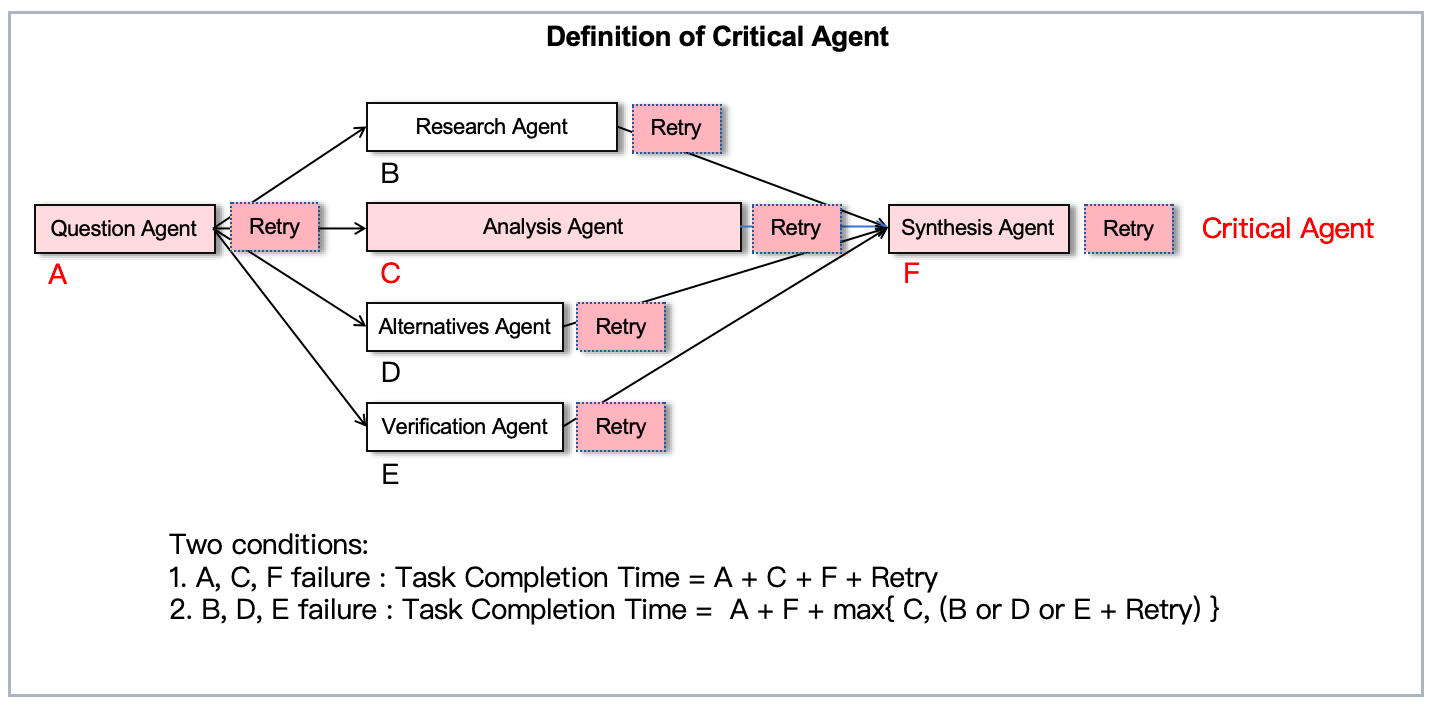
\includegraphics[width=0.88\textwidth]{Figures/critical_agent_definition.png}
  \end{figure}

\end{frame}

\begin{frame}{算法 2（1/5）：在线 Segment Placement 问题}
  \small
  \textbf{不是 offline knapsack}：KV 随 prefill/decode 不断 extend radix node。

  \vspace{0.08cm}
  \textbf{Decision epoch} $t$ 在 node 扩展事件触发（新 token 写入、D2H ACK 等）：
  % \[
  %   \mathcal{N}_{t-1} \subseteq \mathcal{N}_t,
  %   \qquad
  %   \Delta\mathcal{N}_t = \mathcal{N}_t \setminus \mathcal{N}_{t-1}.
  % \]

  \vspace{0.06cm}
  每个 segment / chunk $n \in \mathcal{N}_t$：
  \[
    n = (\operatorname{workflow},\,\operatorname{agent},\,\operatorname{size}_t)
  \]
  其中 $\operatorname{size}_t$ 如果是 decode 中的 segment，可能是固定 step.

  \vspace{0.06cm}
  \textbf{候选过滤}（Algo 1）：
  $\mathcal{C}_t = \{ n \in \mathcal{N}_t \mid \operatorname{critical}(n)=1 \}$，
  Non-Critical 恒有 $x_{n,t}=0$。

  \vspace{0.04cm}
  \footnotesize
  每 epoch 对\textbf{新增 KV segment} n 做备份决策；HostBackup 随 write-through 同步延伸。
\end{frame}

\begin{frame}{算法 2（2/5）：Budget 约束与持有状态}
  \small
  Backup partition 在任意 epoch $t$ 满足\textbf{持有约束}（非一次性分配）：
  \[
    \sum_{n \in \mathcal{P}_t} \operatorname{size}^{\mathrm{gpu}}_t(n)
    \le
    M_{\mathrm{Backup}}(t) = \alpha_t M .
  \]

  \vspace{0.06cm}
  $\mathcal{P}_t$：epoch $t$ 已被 GPUReplica ACK 保护的 segment/chunk 集合；
  $\operatorname{size}^{\mathrm{gpu}}_t(n)$：$n$ 在 GPU 侧实际占用的 unique token 数。

  \vspace{0.08cm}
  \textbf{在线演化}：
  \begin{itemize}
    \item \textbf{Admit}：新 KV segment n 到达，$U(n,t)>0$ 且 budget 有余量
    \item \textbf{Evict}：budget 不足时，淘汰当前 $\mathcal{P}_t$ 中 $\rho$ 最低的条目
    \item \textbf{Invalidate}：Agent 结束，删除 $\mathcal{P}_t$ 中的条目
  \end{itemize}

  \vspace{0.04cm}
  \footnotesize
  HostBackup 不占 $M_{\mathrm{Backup}}$；GPUReplica 才计入上述持有约束。
\end{frame}

\begin{frame}{算法 2（3/5）：Recovery 价值}
  \small
  GPUReplica 保护的\textbf{收益}：failure 时相对 HostBackup restore 能节省多少时延。

  \vspace{0.08cm}
  \[
    V_g(n,t)
    =
    w(n)
    \cdot
    \bigl(
      C_{\mathrm{restore}}^{\mathrm{host}}(|n|, t)
      -
      C_{\mathrm{restore}}^{\mathrm{gpu}}(g, |n|, t)
    \bigr)
  \]

  \vspace{0.06cm}
  \scriptsize
  \renewcommand{\arraystretch}{1.12}
  \begin{tabular}{p{0.30\textwidth}p{0.62\textwidth}}
    \toprule
    项 & 含义 \\
    \midrule
    $w(n)$ & Algo 1 Critical 权重（main / long-decode / fan-out） \\
    $C_{\mathrm{restore}}^{\mathrm{host}}$ & failure 后从 HostBackup restore（H2D）的时延 \\
    $C_{\mathrm{restore}}^{\mathrm{gpu}}(g)$ & failure 后复用 GPUReplica 中的 KV，zero-copy 几乎为 0 \\
    \bottomrule
  \end{tabular}

  \vspace{0.08cm}
  \footnotesize
\end{frame}

\begin{frame}{算法 2（4/5）：Backup 成本}
  \small
  GPUReplica 保护的\textbf{代价}：主动 copy 与 backup HBM 占用。

  \vspace{0.08cm}
  \[
    C_{\mathrm{backup}}^g(n,t)
    =
    C_{\mathrm{copy}}^g(n,t)
    +
    C_{\mathrm{hbm}}^g(n,t)
  \]

  \vspace{0.06cm}
  \scriptsize
  \renewcommand{\arraystretch}{1.12}
  \begin{tabular}{p{0.28\textwidth}p{0.64\textwidth}}
    \toprule
    项 & 含义 \\
    \midrule
    $C_{\mathrm{copy}}^g$ & 复制到 peer $g$ 的 P2P share / 时延（随 locality 变化） \\
    $C_{\mathrm{hbm}}^g$ & peer $g$ 的 Backup partition（$\alpha_t M_g$）占用成本 \\
    \bottomrule
  \end{tabular}

  \vspace{0.10cm}
  对每个候选 peer $g$，计算：
  \[
    U_g(n,t) = V_g(n,t) - C_{\mathrm{backup}}^g(n,t),
    \qquad
    \rho_g(n,t) = \frac{U_g(n,t)}{|n|}.
  \]

  \vspace{0.04cm}
  \footnotesize
  HostBackup 为固定 write-through 底座，不计入 $C_{\mathrm{backup}}^g$。
\end{frame}

\begin{frame}{算法 2（5/5）：Peer 选择与 Event-Driven Admission}
  \small
  \textbf{Peer 选择}：在 healthy peer 集合 $\mathcal{G}_t$ 上取 value-density 最大者：
  \[
    g_t^* = \arg\max_{g \in \mathcal{G}_t} \rho_g(n,t),
    \qquad
    U^* = U_{g_t^*}(n,t).
  \]

  \vspace{0.08cm}
  \textbf{Online decision-making}（每个新增 Radix node / KV Segment n）：
  \begin{enumerate}
    \item 对每个 $g \in \mathcal{G}_t$ 计算 $\rho_g(n,t)$
    \item 选 $g_t^* = \arg\max_g \rho_g$；若 $U^*>0$ 且 $g_t^*$ 有 budget $\rightarrow$ \textbf{admit}
    \item 否则若 $\rho_{g_t^*}$ 高于 $\mathcal{P}_t$ 中最低 $\rho$ $\rightarrow$ \textbf{replace/evict}
  \end{enumerate}

  \vspace{0.06cm}
  \footnotesize
  不同 peer 通过 $C_{\mathrm{restore}}^{\mathrm{gpu}}(g)$ 与 $C_{\mathrm{backup}}^g$ 影响 $\rho_g$；最终 backup 落在 $\rho_g$ 最高的 peer 上。
\end{frame}

\begin{frame}{算法 3：MDP 决定 Backup HBM 比例 $\alpha_t$}
  \small
  对 GPU $g$，AegisKV 把可控 HBM budget $M_g$ 划分为：

  \vspace{0.10cm}
  \[
    M_{\mathrm{Backup}}(g,t) = \alpha_{g,t} M_g,
    \qquad
    M_{\mathrm{Inference}}(g,t) = (1-\alpha_{g,t})M_g .
  \]

  \vspace{0.10cm}
  \begin{block}{Key Trade-off}
    1. Workload ↑ or Failure ↓ -> $\alpha$ ↓ \\
    2. Workload ↓ or Failure ↑ -> $\alpha$ ↑
  \end{block}

  \vspace{0.10cm}
  \footnotesize
  全局 action 是 $\boldsymbol{\alpha}_t=(\alpha_{1,t},\ldots,\alpha_{G,t})$
\end{frame}

\begin{frame}{算法 3：MDP 决定 Backup HBM 比例 $\alpha_t$}
  \small
  在线控制器可以写成 MDP(Markov Decision Process)\cite{yu2026poolcachesadaptivehbm}：

  \vspace{0.04cm}
  \[
    (\mathcal{S},\mathcal{A},\mathcal{P},\mathcal{R},\gamma),
    \qquad
    J(\pi)=\mathbb{E}_{\pi}\left[\sum_{t=0}^{\infty}\gamma^t r_t\right].
  \]

  \vspace{-0.05cm}
  \scriptsize
  \renewcommand{\arraystretch}{1.10}
  \begin{tabular}{p{0.15\textwidth}p{0.72\textwidth}}
    \toprule
    状态 $\mathcal{S}$ 分量 & AegisKV 中的含义 \\
    \midrule
    $h_t$ & Request pressure \\
    $k_t$ & Inference partition 中的 KV / prefix hit rate \\
    $e_t$ & candidate retry tokens 上的 effective backup coverage \\
    $L_t$ & Context length 或 token-length pressure \\
    $\alpha_t$ & backup/inference allocation ratio \\
    \bottomrule
  \end{tabular}

\end{frame}

\begin{frame}{Self Reflection}
  \small
  \begin{columns}[T,onlytextwidth]
    \begin{column}{0.45\textwidth}
      \begin{block}{Presentation}
        \footnotesize
        上次 RcLLM 那篇论文的 presentation 准备得太赶，导致最终完成度和表达效果都不够好。

        \vspace{0.06cm}
        后续需要更早开始整理故事线、核心贡献和关键图，避免只在 deadline 前做材料拼接。
      \end{block}

      \vspace{0.08cm}
      \begin{block}{Research}
        \footnotesize
        Research 不应该直接跳到实现，而应先把理论分析和真实物理测量做扎实，再收敛出可解释、可验证的 solution。
      \end{block}
    \end{column}

    \begin{column}{0.52\textwidth}
      \centering
      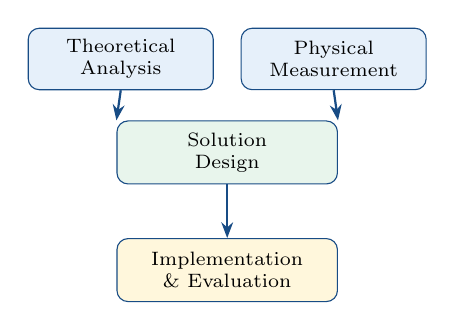
\begin{tikzpicture}[
        node distance=0.52cm and 0.34cm,
        box/.style={draw=hkblue, fill=softblue, rounded corners,
                    align=center, font=\scriptsize, inner sep=4pt,
                    minimum width=2.35cm, minimum height=0.78cm},
        sol/.style={draw=hkblue, fill=softgreen, rounded corners,
                    align=center, font=\scriptsize, inner sep=4pt,
                    minimum width=2.80cm, minimum height=0.80cm},
        impl/.style={draw=hkblue, fill=softyellow, rounded corners,
                     align=center, font=\scriptsize, inner sep=4pt,
                     minimum width=2.80cm, minimum height=0.80cm},
        arr/.style={-{Stealth[length=2mm]}, thick, draw=hkblue}
      ]
        \node[box] (theory) {Theoretical\\Analysis};
        \node[box, right=of theory] (measure) {Physical\\Measurement};
        \node[sol, below=0.78cm of $(theory)!0.5!(measure)$] (solution) {Solution\\Design};
        \node[impl, below=0.68cm of solution] (implementation) {Implementation\\\& Evaluation};

        \draw[arr] (theory.south) -- (solution.north west);
        \draw[arr] (measure.south) -- (solution.north east);
        \draw[arr] (solution) -- (implementation);
      \end{tikzpicture}

      \vspace{0.10cm}
      \footnotesize
      \textbf{Principle:} measure before optimizing; analyze before coding.
    \end{column}
  \end{columns}
\end{frame}

\end{document}
